\documentclass[12pt, letterpaper]{article}
\usepackage[utf8]{inputenc}
\usepackage[left = 2cm, right = 2cm, top = 2.5cm, bottom = 2.5cm]{geometry}
\usepackage{amsthm}
\usepackage{amsfonts}
\usepackage{amsmath}
\usepackage{amssymb}
\usepackage{graphicx}
\usepackage[T1]{fontenc}
\graphicspath{{images/}}

\author{Hernández Ferreiro Enrique Ehecatl (315020904) \\
        López Soto Ramses Antonio (315319974) \\
        Miguel Torres Eric Giovanni (315230190) \\
        Quintero Villeda Erik (315199345)}

\title{Tarea 4: Álgebra Relacional \\
       {\small Fudamentos de Bases de Datos}}

\date{07 de octubre de 2019}

\begin{document}
    \maketitle

    \begin{itemize}

        \item[1.]   Para el \textbf{problema 2} (tarea 3) que transformaste a 
                    \textbf{Modelo Relacional} escribe una expresión en 
                    \textbf{álgebra relacional} para cada una de las siguientes 
                    consultas:

                    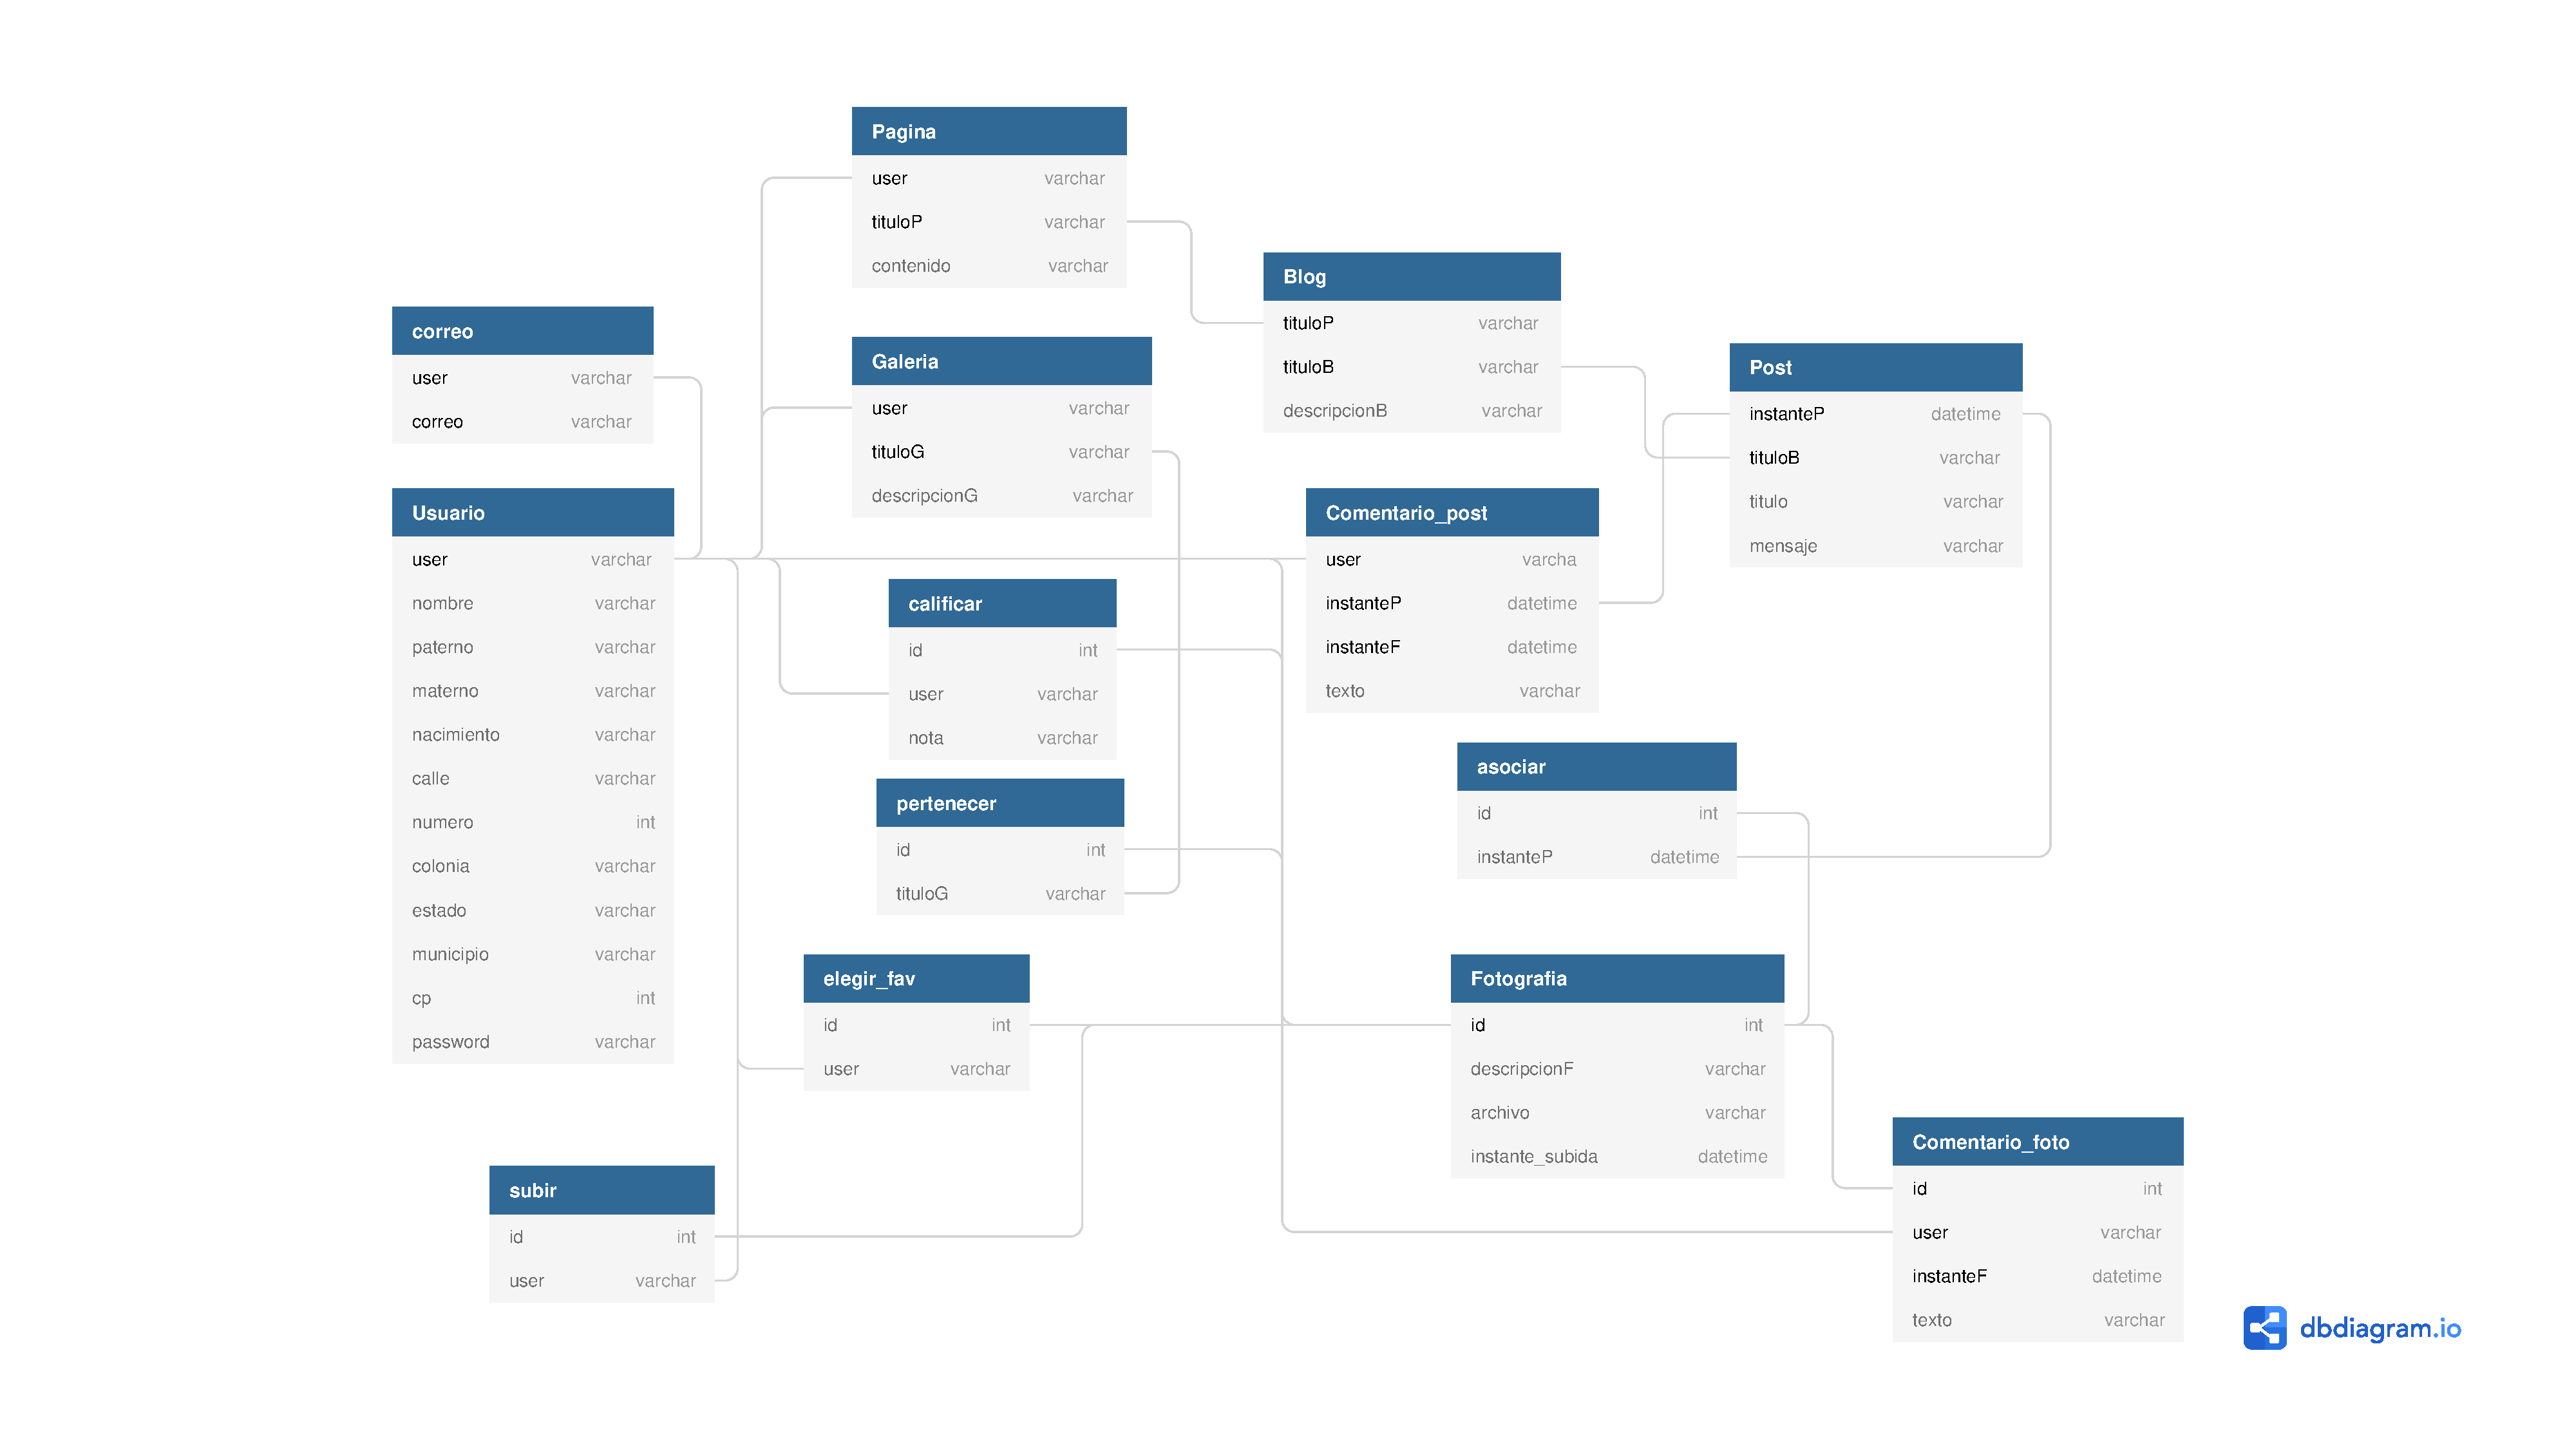
\includegraphics[scale=0.35]{Facebook.png}

                    \newpage

            \begin{itemize}

                \item[\textbf{a.}]   Toda la información de los usuarios que tienen una 
                            página, pero no incluyen blog. 

                            \begin{center}
                                $Usuario \Join (Pagina - Blog)$
                            \end{center}   
                            
                \item[\textbf{b.}]   Una relación que muestre el número total de 
                            fotografías que se han subido por usuario.

                            \begin{center}
                                $\pi_{user, numFotos} ((\gamma_{count(archivo) \rightarrow numFotos} (Fotografia)) \Join Usuario)$    
                            \end{center}    
                            

                \item[\textbf{c.}]   El usuario que más comentarios ha realizado en 
                            fotos.
                            
                            \begin{center}
                                $\pi_{user, numCom}((\gamma_{count(textoF) \rightarrow numCom} (Comentario\_foto)) \Join Usuario)$  
                            \end{center}    

                \item[\textbf{d.}]   Un reporte que muestre por usuario y por álbum 
                            (galería) el total de fotos que se han subido al 
                            sitio. 

                            \begin{center}
                                $\pi_{user, tituloG, totalFotos}((\gamma_{count(archivo) \rightarrow totalFotos} (Fotografia)) \Join Usuario \Join Galeria)$
                            \end{center}

                \item[\textbf{e.}]   La fotografía con más "me gusta" por usuario. 
                 
                            \begin{center}
                                $\pi_{user, numLikes}((\gamma_{max(user) \rightarrow numLikes}(elegir\_fav)) \Join Fotogrfia \Join Usuario)$
                            \end{center}

            \end{itemize} 

        \item[2.-]  Si tienes el siguiente esquema para una Base de Datos: 
                    \vspace{.3cm}
                    
                    \includegraphics[scale=0.5]{HP.png}
        
                    Los fabricantes y los números de modelo se limpiaron, 
                    pero los datos son típicos de los productos a la venta a 
                    principios de 2007. Escribe \textbf{expresiones en álgebra 
                    relacional} para responder las siguientes consultas. Deberás
                    comprobar cada una de ellas en \textbf{RelaX} y agregar en 
                    cada inciso una captura de pantalla con el resultado obtenido.

                    \newpage

            \begin{itemize}

                \item[\textbf{a.}]  ¿Qué modelos de PC tienen una velocidad entre
                                    3 y 3.5 GHz? 

                                    \begin{center}
                                        $\pi_{model}(\sigma_{speed \geq 3 \hspace{.1cm} \land \hspace{.1cm} speed \leq 3.5} (PC))$\vspace{.3cm}

                                        \includegraphics[scale=0.3]{a.png}
                                    \end{center}


                \item[\textbf{b.}]  ¿Qué fabricantes producen computadoras 
                                    portátiles con un dico duro de menos 100 GB?
                                    
                                    \begin{center}
                                        $\pi_{maker}(Product \Join (\sigma_{hd < 100} (Laptop)))$\vspace{.3cm}

                                        \includegraphics[scale=0.3]{b.png}
                                    \end{center}
                
                                    \newpage
                \item[\textbf{c.}]  Encontrar el número de modelo y el precio de 
                                    todos los productos (de cualquier tipo) 
                                    fabricados por el fabricante B.

                                    \begin{center}
                                        $(\pi_{model,price}(\sigma_{maker = 'B'} (Product \Join PC))) \cup (\pi_{model,price}(\sigma_{maker = 'B'} (Product \Join Laptop))) 
                                        \cup (\pi_{Product.model,price}(\sigma_{maker = 'B'} (Product \Join_{Product.model = Printer.model} Printer)))$\vspace{.3cm}

                                        \includegraphics[scale=0.25]{c.png}
                                    \end{center}

                \item[\textbf{d.}]  Encontrar toda la información de los fabricantes 
                                    que produzcan los tres tipos de productos. 
                                    
                                    \begin{center}
                                        $\pi_{maker, Product.model,Product.type}(((\pi_{maker}(\sigma_{type='laptop'}(Product))) \cap (\pi_{maker}(\sigma_{type='pc'}(Product)))  \cap 
                                        (\pi_{maker}(\sigma_{type='printer'}(Product)))) \Join Product)$\vspace{.3cm}

                                        \includegraphics[scale=0.2]{d.png}
                                    \end{center}

                \item[\textbf{e.}]  Encontrar los números de modelo de todas las 
                                    impresoras láser a color.

                                    \begin{center}
                                        $\pi_{model}(\sigma_{type='laser'\hspace{.1cm}\land\hspace{.1cm} color=ture}(Printer))$\vspace{.3cm}

                                        \includegraphics[scale=0.26]{e.png}
                                    \end{center}

                \item[\textbf{f.}]  Encontrar toda la información de los fabricantes 
                                    que venden laptops pero no PC's.

                                    \begin{center}
                                        $\sigma_{type='laptop'}(((\pi_{maker}(\sigma_{type='laptop'}(Product))) - (\pi_{maker}(\sigma_{type='laptop'}(Product)))) \Join 
                                        Product \Join Laptop)$ \vspace{.3cm}

                                        \includegraphics[scale=0.26]{f.png}
                                    \end{center}

                \newpage 

                \item[\textbf{g.}]  Encontrar los tamaños de disco duro que están 
                                    presentes en dos o más PC's. 

                                    \begin{center}
                                        $\pi_{hd} (\sigma_{numHD > 1}(\gamma_{hd; count(hd)\rightarrow numHD}(PC)))$\vspace{.3cm}

                                        \includegraphics[scale=0.25]{g.png}
                                    \end{center}

                \item[\textbf{h.}]  Encontrar toda la información de las PC's que 
                                    tienen la misma velocidad y RAM. 

                                    \begin{center}
                                        $PC \Join ((\pi_{speed, ram} (\sigma_{numRAM > 1}(\gamma_{speed, ram; count(ram)\rightarrow numRAM}(PC)))) \cup 
                                        (\pi_{speed, ram}(\sigma_{numSpeed > 1}(\gamma_{speed,ram; count(speed)\rightarrow numSpeed}(PC)))))$ \vspace{.3cm}

                                        \includegraphics[scale=0.25]{h.png}
                                    \end{center}

                \newpage

                \item[\textbf{i.}]  Encontrar aquellos fabricantes de mínimo dos 
                                    computdoras diferentes (PC o laptop) con 
                                    velocidades de al menos 2.80 GHz.

                                    \begin{center}
                                        $(\pi_{maker}(\sigma_{speed \geq 2.8}(Product \Join Laptop))) \cup (\pi_{maker}(\sigma_{speed\geq 2.8}(Product \Join PC)))$ \vspace{.3cm}

                                        \includegraphics[scale=0.25]{i.png}
                                    \end{center}

                \item[\textbf{j.}]  Encontrar el fabricante de la computdora 
                                    (PC o laptop) con la velocidad más alta 
                                    posible. 

                                    \begin{center}
                                        $(\pi_{maker}(Product \Join (Laptop \Join_{speed = maxSL} (\gamma_{max(speed)\rightarrow mxSL}(Laptop))))) \cup 
                                        (\pi_{maker}(Product \Join (PC \Join_{speed = maxSP} (\gamma_{max(speed)\rightarrow mxSP}(PC)))))$ \vspace{.3cm}

                                        \includegraphics[scale=0.25]{j.png}
                                    \end{center}

                \item[\textbf{k.}]  Encontrar los fabricantes de PC con al menos 
                                    tres velocidades diferentes.

                                    \begin{center}
                                        $(\pi_{maker}(\sigma_{numS \geq 3} (\gamma_{maker; count(speed) \rightarrow numS}(PC \Join Product)))) - 
                                        (\pi_{maker}(\sigma_{maker='B'}(PC \Join Product)))$ \vspace{.3cm}

                                        \includegraphics[scale=0.25]{k.png}
                                    \end{center}

                \item[\textbf{l.}]  Encontrar los fabricantes que venden 
                                    exactamente tres modelos diferentes de PC. 
                                    
                                    \begin{center}
                                        $\pi_{maker}(((\gamma_{count(model)\rightarrow numMod}(\sigma_{maker='A'}(\pi_{maker,model}(Product \Join PC)))) \Join 
                                        (\sigma_{maker='A'}(Product \Join PC))) \cup ((\gamma_{count(model)\rightarrow numMod}(\sigma_{maker='B'}(\pi_{maker,model}(Product \Join PC)))) \Join 
                                        (\sigma_{maker='B'}(Product \Join PC))) \cup ((\gamma_{count(model)\rightarrow numMod}(\sigma_{maker='C'}(\pi_{maker,model}(Product \Join PC)))) \Join 
                                        (\sigma_{maker='C'}(Product \Join PC))) \cup ((\gamma_{count(model)\rightarrow numMod}(\sigma_{maker='D'}(\pi_{maker,model}(Product \Join PC)))) \Join 
                                        (\sigma_{maker='D'}(Product \Join PC))) \cup ((\gamma_{count(model)\rightarrow numMod}(\sigma_{maker='E'}(\pi_{maker,model}(Product \Join PC)))) \Join 
                                        (\sigma_{maker='E'}(Product \Join PC))) \cup ((\gamma_{count(model)\rightarrow numMod}(\sigma_{maker='G'}(\pi_{maker,model}(Product \Join PC)))) \Join 
                                        (\sigma_{maker='F'}(Product \Join PC))) \cup ((\gamma_{count(model)\rightarrow numMod}(\sigma_{maker='H'}(\pi_{maker,model}(Product \Join PC)))) \Join 
                                        (\sigma_{maker='H'}(Product \Join PC))))$ \vspace{.3cm}

                                        \includegraphics[scale=0.35]{l.png}
                                    \end{center}

                \newpage

                \item[\textbf{m.}]  Encontrar toda la información de la laptop 
                                    más cara. 

                                    \begin{center}
                                        $Laptop \Join_{price=maxPrice}(\gamma_{max(price)\rightarrow maxPrice}(Laptop))$ \vspace{.3cm}

                                        \includegraphics[scale=0.25]{m.png}
                                    \end{center}

                \item[\textbf{n.}]  Crear un reporte que muestre por fabricante, 
                                    el número de productos que tiene de cada 
                                    tipo. 

                                    \begin{center}
                                        $(\pi_{maker, numPC, numLaptop, numPrinter} (((\gamma_{count(type)\rightarrow numPC}(\sigma_{maker='A' \land type = 'pc'} (Product))) \Join (\sigma_{maker=''A} (Product))) \Join 
                                        ((\gamma_{count(type)\rightarrow numLaptop}(\sigma_{maker='A' \land type = 'laptop'} (Product))) \Join (\sigma_{maker=''A} (Product))) \Join 
                                        ((\gamma_{count(type)\rightarrow numPrinter}(\sigma_{maker='A' \land type = 'printer'} (Product))) \Join (\sigma_{maker='A'} (Product)))) \cup 
                                        (\pi_{maker, numPC, numLaptop, numPrinter} (((\gamma_{count(type)\rightarrow numPC}(\sigma_{maker='B' \land type = 'pc'} (Product))) \Join (\sigma_{maker='B'} (Product))) \Join 
                                        ((\gamma_{count(type)\rightarrow numLaptop}(\sigma_{maker='B' \land type = 'laptop'} (Product))) \Join (\sigma_{maker='B'} (Product))) \Join 
                                        ((\gamma_{count(type)\rightarrow numPrinter}(\sigma_{maker='B' \land type = 'printer'} (Product))) \Join (\sigma_{maker='B'} (Product)))) \cup 
                                        (\pi_{maker, numPC, numLaptop, numPrinter} (((\gamma_{count(type)\rightarrow numPC}(\sigma_{maker='C' \land type = 'pc'} (Product))) \Join (\sigma_{maker='C'} (Product))) \Join 
                                        ((\gamma_{count(type)\rightarrow numLaptop}(\sigma_{maker='C' \land type = 'laptop'} (Product))) \Join (\sigma_{maker='C'} (Product))) \Join 
                                        ((\gamma_{count(type)\rightarrow numPrinter}(\sigma_{maker='C' \land type = 'printer'} (Product))) \Join (\sigma_{maker='C'} (Product)))) \cup 
                                        (\pi_{maker, numPC, numLaptop, numPrinter} (((\gamma_{count(type)\rightarrow numPC}(\sigma_{maker='D' \land type = 'pc'} (Product))) \Join (\sigma_{maker='D'} (Product))) \Join 
                                        ((\gamma_{count(type)\rightarrow numLaptop}(\sigma_{maker='D' \land type = 'laptop'} (Product))) \Join (\sigma_{maker='D'} (Product))) \Join 
                                        ((\gamma_{count(type)\rightarrow numPrinter}(\sigma_{maker='D' \land type = 'printer'} (Product))) \Join (\sigma_{maker='D'} (Product)))) \cup 
                                        (\pi_{maker, numPC, numLaptop, numPrinter} (((\gamma_{count(type)\rightarrow numPC}(\sigma_{maker='E' \land type = 'pc'} (Product))) \Join (\sigma_{maker='E'} (Product))) \Join 
                                        ((\gamma_{count(type)\rightarrow numLaptop}(\sigma_{maker='E' \land type = 'laptop'} (Product))) \Join (\sigma_{maker='E'} (Product))) \Join 
                                        ((\gamma_{count(type)\rightarrow numPrinter}(\sigma_{maker='E' \land type = 'printer'} (Product))) \Join (\sigma_{maker='E'} (Product)))) \cup 
                                        (\pi_{maker, numPC, numLaptop, numPrinter} (((\gamma_{count(type)\rightarrow numPC}(\sigma_{maker='F' \land type = 'pc'} (Product))) \Join (\sigma_{maker='F'} (Product))) \Join 
                                        ((\gamma_{count(type)\rightarrow numLaptop}(\sigma_{maker='F' \land type = 'laptop'} (Product))) \Join (\sigma_{maker='F'} (Product))) \Join 
                                        ((\gamma_{count(type)\rightarrow numPrinter}(\sigma_{maker='F' \land type = 'printer'} (Product))) \Join (\sigma_{maker='F'} (Product)))) \cup 
                                        (\pi_{maker, numPC, numLaptop, numPrinter} (((\gamma_{count(type)\rightarrow numPC}(\sigma_{maker='G' \land type = 'pc'} (Product))) \Join (\sigma_{maker='G'} (Product))) \Join 
                                        ((\gamma_{count(type)\rightarrow numLaptop}(\sigma_{maker='G' \land type = 'laptop'} (Product))) \Join (\sigma_{maker='G'} (Product))) \Join 
                                        ((\gamma_{count(type)\rightarrow numPrinter}(\sigma_{maker='G' \land type = 'printer'} (Product))) \Join (\sigma_{maker='G'} (Product)))) \cup 
                                        (\pi_{maker, numPC, numLaptop, numPrinter} (((\gamma_{count(type)\rightarrow numPC}(\sigma_{maker='H' \land type = 'pc'} (Product))) \Join (\sigma_{maker='H'} (Product))) \Join 
                                        ((\gamma_{count(type)\rightarrow numLaptop}(\sigma_{maker='H' \land type = 'laptop'} (Product))) \Join (\sigma_{maker='H'} (Product))) \Join 
                                        ((\gamma_{count(type)\rightarrow numPrinter}(\sigma_{maker='H' \land type = 'printer'} (Product))) \Join (\sigma_{maker='H'} (Product))))$ \vspace{.3cm}

                                        \includegraphics[scale=0.35]{n.png}
                                    \end{center}

                \item[\textbf{o.}]  Incrementar en un 15\% el tamaño de diaco 
                                    duro de las laptops del fabricante E que 
                                    son menores a 200 GB.

                                    \begin{center}
                                        $\pi_{maker, model, ram, nuevoTamHD \leftarrow hd*1.15, price}(\sigma_{mker='E' \hspace{.1cm} \land \hspace{.1cm} hd < 200}(Product \Join Laptop))$ \vspace{.3cm}

                                        \includegraphics[scale=0.25]{o.png}
                                    \end{center}

                \item[\textbf{p.}]  Borrar todas las impresoras de inyección 
                                    de tinta.

                                    \begin{center}
                                        $(\pi_{model, color, type, price}(Printer))- (\sigma_{type='ink-jet'}(Printer))$ \vspace{.3cm}

                                        \includegraphics[scale=0.25]{p.png}
                                    \end{center}

                \item[\textbf{q.}]  Insertar un nuevo fabricante que produzca 
                                    los tres tipos de productos e insertar al 
                                    menos un producto de cada tipo para este 
                                    fabricante. \vspace{.2cm}

                                    $product$ $= \{$ $maker:string$ \hspace{.2cm} $model:number$ \hspace{.2cm} $type:string$ \vspace{.1cm}

                                    \hspace{3.5cm} $I$ \hspace{2.2cm} $2004$ \hspace{1.8cm} $laptop$ \vspace{.1cm}

                                    \hspace{3.5cm} $I$ \hspace{2.2cm} $1014$ \hspace{2.2cm} $pc$ \vspace{.1cm}

                                    \hspace{3.5cm} $I$ \hspace{2.2cm} $3008$ \hspace{1.8cm} $printer$ \vspace{.1cm}

                                    $\}$ \vspace{.5cm}

                                    $pc$ $= \{$ $model:number$ $speed:number$ $ram:number$ $hd:number$ $price:number$ \vspace{.1cm}

                                    \hspace{2cm} $2004$ \hspace{2cm} $1.80$ \hspace{1.5cm} $300$ \hspace{1.5cm} $250$ \hspace{1.7cm} $1235$ \vspace{.1cm}

                                    $\}$ \vspace{.5cm}

                                   {\scriptsize $laptop$ $= \{$ $model:number$ $speed:number$ $ram:number$ $hd:number$ $screen:number$ $price:number$ \vspace{.1cm}

                                    \hspace{2cm} $1014$ \hspace{1.3cm} $2.60$ \hspace{1.3cm} $450$ \hspace{1.3cm} $500$ \hspace{1.3cm} $25.2$ \hspace{1.4cm} $2067$ \vspace{.1cm}

                                    $\}$  }\vspace{.5cm}

                                    $printer$ $= \{$ $model:number$ \hspace{.2cm} $color:boolen$ \hspace{.2cm} $type:string$ \hspace{.2cm} $price:number$ \vspace{.1cm}

                                    \hspace{3cm} $3008$ \hspace{2cm} $true$ \hspace{1.8cm} $laser$ \hspace{1.5cm} $2045$  \vspace{.1cm}

                                    $\}$ \vspace{.5cm}

                                    \newpage

                                    \begin{center}
                                        $Product \cup product$ \vspace{.3cm}

                                        \includegraphics[scale=0.22]{q1.png}
                                        \includegraphics[scale=0.22]{q11.png}
                                    \end{center}

                                    \begin{center}
                                        $(Product \cup product) \Join (PC \cup pc)$\vspace{.3cm}

                                        \includegraphics[scale=0.22]{q2.png}
                                        \includegraphics[scale=0.22]{q22.png}
                                    \end{center}

                                    \begin{center}
                                        $(Product \cup product) \Join (Laptop \cup laptop)$\vspace{.3cm}

                                        \includegraphics[scale=0.24]{q3.png}
                                        \includegraphics[scale=0.24]{q33.png}
                                    \end{center}

                                    \begin{center}
                                        $(Product \cup product) \Join_{Product.model=Printer.model} (Printer \cup printer)$\vspace{.3cm}

                                        \includegraphics[scale=0.24]{q4.png}
                                    \end{center}

            \end{itemize} 
            
    \end{itemize}
    
\end{document}
